\documentclass[a4paper, 12pt]{article}
% Options possibles : 10pt, 11pt, 12pt (taille de la fonte)
% oneside, twoside (recto simple, recto-verso)
% draft, final (stade de développement)
\usepackage[utf8]{inputenc} % LaTeX, comprends les accents !
\usepackage[T1]{fontenc} % Police contenant les caractères français
\usepackage{geometry} % Définir les marges
\usepackage[francais]{babel} % Placez ici une liste de langues, la
% dernière étant la langue principale
\usepackage{graphicx}
\usepackage{verbatim}
\usepackage{float}
\usepackage{booktabs}
\usepackage{amsmath}
\usepackage{amsfonts}
\usepackage{multirow}
\geometry{left=2.2cm,right=2.2cm,top=2.5cm,bottom=2.5cm}
% \pagestyle{headings} % Pour mettre des entêtes avec les titres
% des sections en haut de page
%\include[dvips]{graphics}
\title{Kohonen Map Project Report \\ \vspace{0.5cm} \large Unsupervised and Reinforcement Learning in Neural Networks}
\author{Han JU, Hao Ren}
\date{\today}
\begin{document}
\maketitle
\section{Learning rate and convergence}
In this part, we start with a Khohonen network of 6x6 neurons and use a Gaussian neighborhood function with standard deviation $\sigma = 3$.
We have tried several learning rates, the observations are showed as below:
\begin{enumerate}
\item eta = 0.01 : numbre of iterations = 4
\item eta = 0.001 : numbre of iterations = 24
\item eta = 0.0001 : numbre of iterations = 48
\end{enumerate}

The result is exactly the same to our intuition, small learning rates cause the algorithm to converge slower, while the larger ones help the algorithm to converge faster. However, we cannot tell which one is better. As we know, the final solution of the small learning rate will be more stationary, but it might be stuck in local minima, while the large one might make the weights fail to converge.

For the three learning rate, the resulting figures have no big difference, as the one show above. What is important is that the three learning rates all leads to the convergence of the algorithm. So we can conclude that the bigger learning rate has no side-effect in this project. In addition, according to our observation, smaller learning rate doesn't improve our result. That means the quality of the result depends on other parameters which will be discussed in the later section. As a result, we choose eta = 0.01

In the origin matlab code downloaded from the Moodle, there is a
simple convergence rule which just iterate the algorithm as many times
as the number of the data points. In most of the case, it is not good enough, as some noticeable changes are observed. In order to improve this, we have defined a new convergence condition which is described as following:
\begin{equation}
  \frac{\Vert centers_{n+1} - centers_n\Vert}{\Vert centers_n \Vert}
  < 0.01
\end{equation}
where 0.01 is a converge criterion which can be chosen as needed and each row of the matrix centers is one of the prototypes.

In our convergence rule, every iteration use all the data points to calculate the centers. After each iteration, the convergence condition will be tested which will decide whether the algorithm will go on or not. If the change is small enough between the centers of two successive iterations, we can conclude that the algorithm converges. Mathematically, that is to say the norm of the difference of the two centers matrix is sufficient small (relative to the norm of the previous one).
\section{Visualization and prototypes}
\begin{figure}[h]
\centering
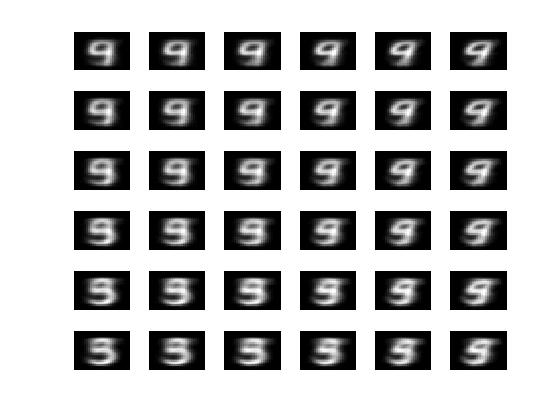
\includegraphics[scale=0.4]{../figure/sigma3eta001size6.jpg}
\caption{Visualization of prototypes}
\end{figure}
Figure 1 is the Visualization of the prototypes in the map with standard parameters ($eta = 0.01$, $\sigma = 3$) for the digit set $3,
4, 5, 9$. From the figure we can't tell much difference between the prototypes. We can say that under this setting, the resulting map is not of a high quality.
\section{Assignment method}
In this step, we need a method to automatically assign the proper digit to each prototype that we found by executing the Kohonen map algorithm. An obvious idea is to look at the labels of the training data points that are close to the prototype, then decide the its label according to the majority in its surroundings. In fact, this task has a similarity with the $k$ nearest neighbor classification algorithm, which assigns a label to a data sample based on the majority of its $k$ nearest neighbors. So we decided to use the kNN method.
Before we apply this method directly to the problem, however, we need to determine the parameter, $k$, of this algorithm. Intuitively, this parameter depends on our training data, which covers the hand writing samples of the four chosen digits. So we do firstly a cross validation on kNN models with distinct $k$ values (ranging from 3 to 300), which results in $k$ equals 5.
Once the parameter is fixed, the application of kNN to the problem is fairly straightforward.
As a result, we have a matrix which contains the assigned digit to the corresponding prototype of the resulting figure matrix, as in figure 2.
\begin{figure}
  \centering
  \begin{minipage}[c]{0.5\textwidth}
    \centering
    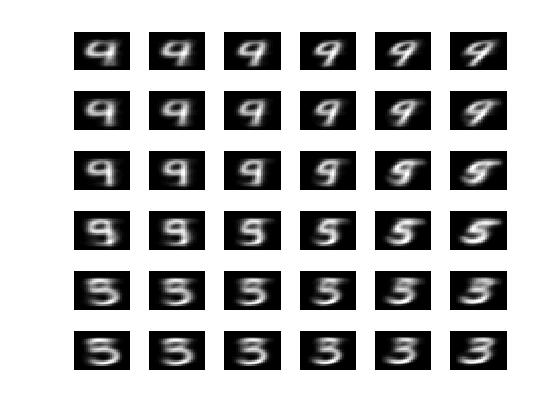
\includegraphics[scale=0.4]{../figure/assign.jpg}
  \end{minipage}%
  \begin{minipage}[c]{0.5\textwidth}
    \centering
    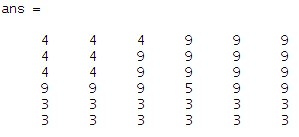
\includegraphics[scale=0.8]{../figure/assignMatrix.jpg}
  \end{minipage}
  \caption{Prototypes and assigned digits}
\end{figure}
\section{$\sigma$ and map size}
In this section we will discuss the role of the width of the neighborhood function and the size of the Kohonen map.
\subsection{Constant $\sigma$ and map size}
With different $\sigma$ and size of map, we will get different
resulting matrix. In order to describe and compare the quality of the
resulting map, we come up with a way to define the error rate:
\begin{enumerate}
\item For each data point, we find the prototype which is closest to
  the data point, and assign the digit of the prototype to the data
  point
\item compare the digits of the data points to the labels, if the
  digit is not the same, we count this as an error.
\item finally, we get the error rate: $\dfrac{\#error}{\#dataPoints}$
\end{enumerate}
For the test scheme, we firstly cut out dataset into training and test
set with a $9:1$ ratio. Kohonen maps are constructed with the
training data, then we apply them to classify data points in the test
set to calculate the error rate mentioned earlier. In this way, the
error rate can be regarded as a reliable measure of the map quality.
We have tried $\sigma = 1, 3, 5$ and $sizeK = 6, 7, 8$, the result is showed as table-1:
\begin{table}[!hbp]
\centering
\begin{tabular}{|c|c|c|c|}
\hline
 & $\sigma = 1$ & $\sigma = 3$ & $\sigma = 5$\\
\hline
$sizeK = 6$ &  0.4665 & 0.4790 & 0.5360\\
\hline
$sizeK = 8$ & 0.3925 & 0.5270 & 0.5505\\
\hline
$sizeK = 10$ & 0.2635 & 0.5165 & 0.5765\\
\hline
\end{tabular}
\caption{error rate with different $\sigma$ and $sizeK$}
\end{table}
As a result, the optimal width does not depend on the size of the
Kohonen map. For different sizes of the map, the smaller sigma is ,
the better quality the result has. That means the optimal sigma is
always the smaller one, no matter how the size of the map
changes. With the increase of the size of the Kohonen map, the quality
is improved. An intuitive interpretation of this is that each prototype
covers fewer and fewer data points, which makes the prototype's
position become more and more accurate during the convergence.

In fact, the sigma controls the strength and range of the neighborhood effect of the points of the map. With a small sigma, the algorithm is essentially the competitive learning algorithm, with possible dead units, because the initialization might not be good enough. With big sigmas, all prototypes learn the same thing, i.e. the center of the points.

For the map size, we've found that when width is small, it has a
significant influence on the quality. However, when $\sigma$ is
bigger, the quality is dominated by $\sigma$, changing de map
size doesn't change much the error rate.

A proper size of the Kohonen map helps to prevent over fitting. Especially, in the unsupervised learning, it is better to fitting the data with a more or less regular grid that captures the essence of the underlying distribution than using a naive clustering algorithm with so many free parameters.
\subsection{Variable $\sigma$}
Finally, we adopt another approach that is to decrease the
neighborhood width parameter with iterations.
We decrease this parameter with following scheme:
\begin{equation}
  \sigma (n) = \sigma _0 \, exp(-\frac{n}{\tau _1}) \qquad n = 0, 1, 2 ...
\end{equation}
moreover, we have
\begin{equation}
  \tau _1 = \frac{1000}{log \, \sigma _0}
\end{equation}
We fixed the initial width to a large value, say $10$, and the result
map is with very high quality even with a simple visual check. An
interesting point is that if the initial value is not big enough,
we'll have some badly-fitted prototype in the result map. This problem
is probably due to the fact that the neighborhood of the winning
neuron is decreasing with the runtime of the algorithm and if the
initial value is not big enough, some unlucky prototype of the map may
not be updated properly.
\begin{figure}[h]
  \begin{minipage}[c]{0.45\textwidth}
    \begin{figure}[H]
      \centering
      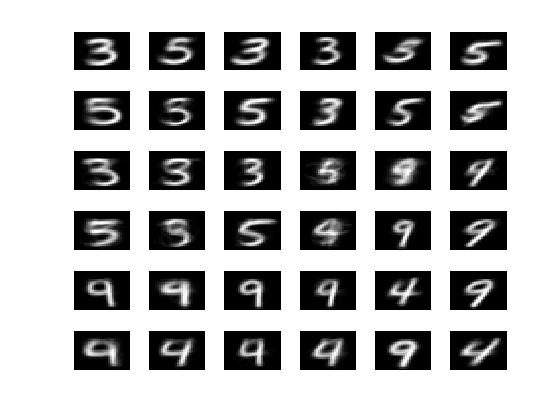
\includegraphics[scale=0.4]{../figure/sigmaLarge.jpg}
      \caption{Variable $\sigma$ with large initial value}
    \end{figure}
  \end{minipage}%
  \hspace{0.5cm}
  \begin{minipage}[c]{0.45\textwidth}
    \begin{figure}[H]
      \centering
      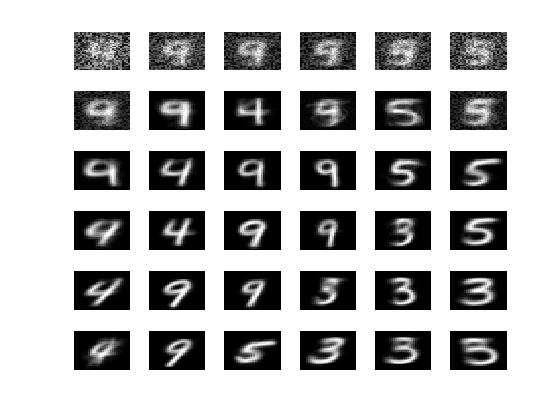
\includegraphics[scale=0.4]{../figure/sigmaSmall.jpg}
      \caption{Variable $\sigma$ with small initial value}
    \end{figure}
  \end{minipage}
\end{figure}
\section{Conclusion}
In this mini-project we've studied the self-organizing map by applying
this technique to a concrete example. Meanwhile, we analyzed
mainly the convergence condition of the map, as well as the influence of its
different parameters to the final result. With this project, we fully
understand the principle of self-organizing maps as a powerful tool in
data analysis.
\end{document}
